\chapter{PHƯƠNG PHÁP LẬP TRÌNH CHO QUY HOẠCH TUYẾN TÍNH}

Trong chương này, chúng tôi trình bày ví dụ minh họa trong việc sử dụng ngôn ngữ lập trình Python và thư viện bộ giải Gurobi\cite{gurobi}.

\section{Cài đặt phần mềm}

Trước tiên, chúng ta cần có sẵn môi trường Python. Sau đó, chúng ta sẽ cài đặt thư viện Gurobi. Gurobi là một trong những công cụ giải quyết tối ưu hóa mạnh mẽ và nhanh nhất và công ty liên tục tung ra các tính năng mới. Câu lệnh cài đặt như sau
\begin{mintedbox}{python}
python -m pip install -i https://pypi.gurobi.com gurobipy==10.0
\end{mintedbox}

\section{Bài toán quy hoạch tuyến tính}

Xem xét một công ty sản xuất sản xuất hai mặt hàng: cốc và đĩa. 
\begin{itemize}
    \item Sau khi làm xong, một chiếc cốc được bán với giá 27 USD và một chiếc đĩa được bán với giá 21 USD.
    \item Để làm ra mỗi chiếc cốc, chi phí vật liệu là 10 USD và nhân công là 14 USD.
    \item Để làm ra mỗi chiếc đĩa, chi phí vật liệu là 9 USD và nhân công là 10 USD.
    \item Để làm ra mỗi chiếc cốc, phải mất 2,2 giờ lao động.
    \item Để làm ra mỗi chiếc đĩa, phải mất 1 giờ lao động.
    \item Hãng có nguồn cung nguyên liệu vô hạn.
    \item Do số lượng công nhân có hạn nên một công ty có tối đa 100 giờ lao động.
    \item Nhu cầu về cốc là không giới hạn nhưng nhu cầu về đĩa là 30 chiếc.
\end{itemize}

Mục tiêu của công ty là tối đa hóa lợi nhuận (doanh thu – chi phí).

\section{Giải bài toán}

\subsection{Bước 1 - Định nghĩa các biến}

\begin{mintedbox}{python}
# Create variables
x1 = m.addVar(name="x1")
x2 = m.addVar(name="x2")
\end{mintedbox}

\subsection{Bước 2 - Định nghĩa hàm mục tiêu}

\begin{mintedbox}{python}
# Set objective
m.setObjective(3*x1 + 2*x2 , GRB.MAXIMIZE)
\end{mintedbox}

\subsection{Bước 3 - Định nghĩa các ràng buộc bất đẳng thức}

\begin{mintedbox}{python}
# Build (sparse) constraint matrix
m.addConstr(2.2*x1 + x2  <= 100, "c1")
m.addConstr(x2  <= 30, "c3")
m.addConstr(x1  >= 0, "c4")
m.addConstr(x2  >= 0, "c5")
\end{mintedbox}

\section{Chương trình hoàn thiện và thực nghiệm}

Toàn bộ mã nguồn và kết quả thực nghiệm

\begin{figure}[h!]
    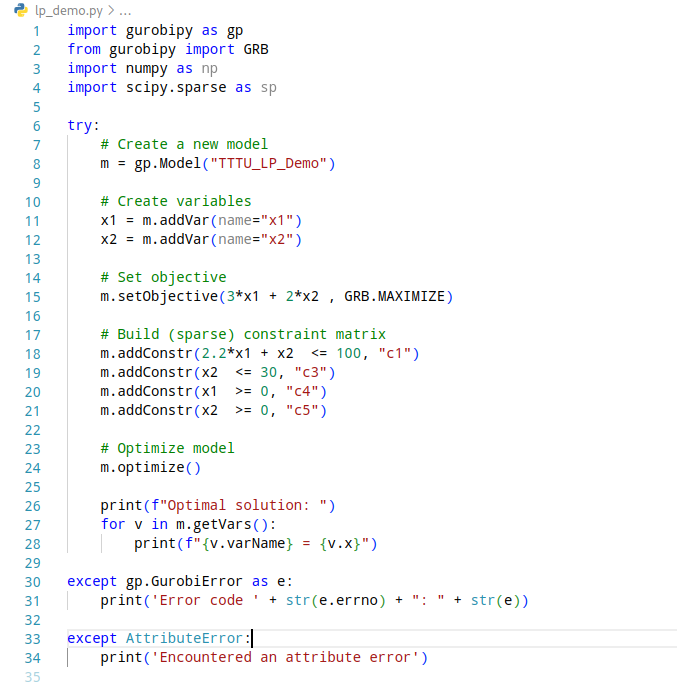
\includegraphics[width=0.85\linewidth]{figures/lp_demo1.png}
    \caption{Mã nguồn chương trình.}
    \label{fig:lp_demo1}
\end{figure}

\begin{figure}[h!]
    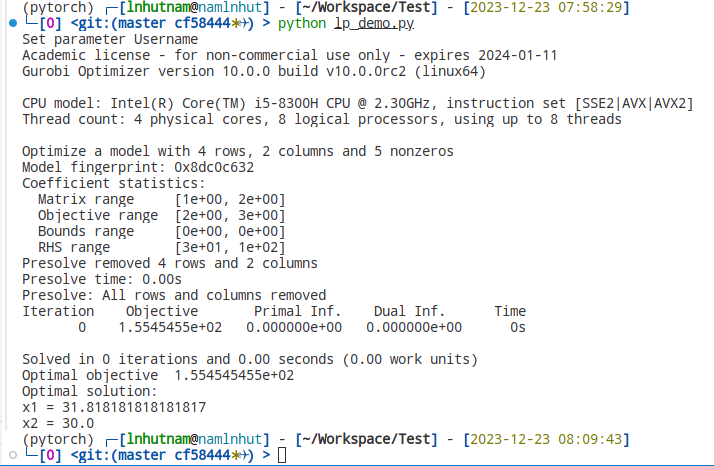
\includegraphics[width=0.85\linewidth]{figures/lp_demo2.png}
    \caption{Kết quả thực nghiệm.}
    \label{fig:lp_demo2}
\end{figure}